\originalchapter{8.09作业九}\label{chap:cm-pset9}
题源: Assignment 9, 2014年11月26日18时截止, 实际题面PDF第2--5页. 以下五题题面按原件中文表述, 解答均为AI独立推导或独立数值复现; OCW未提供这份作业的官方解答. 数值脚本替代原题Mathematica操作, 不读取或执行来源不明的notebook, 模型与原题方程一致.

\begin{exercise}
原题1（10分）. 密度$\rho$、运动黏度$\nu$的水, 在与水平成角$\theta$的无限斜面上形成厚$h$的稳定不可压层流. 表面气压$p_{\rm atm}$. (a) 写适用的Navier--Stokes方程. (b) 由对称性确定速度与压力形式, 给固壁与自由表面边界条件. (c) 求速度和压力分布.
\end{exercise}
\begin{solution}
取$x$沿坡向下、$y$垂直坡面向外, 水层$0\le y\le h$. 坡向及横向平移对称给$\vect v=u(y)\vect e_x$, $p=p(y)$, 连续性自动满足, 对流导数$(\vect v\cdot\nabla)\vect v=0$. 动量式$0=-\nabla p/\rho+\vect g+\nu\nabla^2\vect v$, 两个分量为$\nu u''+g\sin\theta=0$, $p'=-\rho g\cos\theta$. 固壁无滑移$u(0)=0$, 忽略空气切应力时自由面$u'(h)=0$, 另有$p(h)=p_{\rm atm}$. 两次积分得
\[
u(y)=\frac{g\sin\theta}{2\nu}(2hy-y^2),\qquad
p(y)=p_{\rm atm}+\rho g\cos\theta(h-y).
\]
此处$\nu$是运动黏度, 若改用动力黏度$\eta$, 应以$\eta/\rho$代入. 速度最大值$u(h)=gh^2\sin\theta/(2\nu)$, 单位宽流量$Q'=\int_0^h u\dd y=gh^3\sin\theta/(3\nu)$, 可作为量纲核验.
\end{solution}

\begin{exercise}
原题2（15分）. 阻尼摆$\dot\theta=w$, $\dot w=-w/q-\sin\theta$, $q>0$, 固定点$(n\pi,0)$. (a) 线性化. (b) $q=\infty$时解中心与鞍点, 给纯增长/纯衰减方向. (c) 有限$q$在吸引点附近分别解$q>1/2$、$q<1/2$并画相轨道. (d) 给鞍点增长率与增长方向相对$\theta$轴的角.
\end{exercise}
\begin{solution}
写$\eta=\theta-n\pi$, 则$\dot\eta=w$, $\dot w=-w/q-(-1)^n\eta$. 偶$n$对应底部. 无阻尼时$\eta=A\cos t+B\sin t$, $w=-A\sin t+B\cos t$, 相轨道$\eta^2+w^2=A^2+B^2$为中心. 奇$n$有$\eta=Ae^t+Be^{-t}$, $w=Ae^t-Be^{-t}$; 在本册横轴$\eta$、纵轴$w$的坐标中, 增长方向$(1,1)$、衰减方向$(1,-1)$（若依原题将$w$写在前, 两分量同步交换）.

底部特征根$\lambda_\pm=-1/(2q)\pm\sqrt{1/(4q^2)-1}$. $q>1/2$时令$\Omega=\sqrt{1-1/(4q^2)}$, $\eta=e^{-t/(2q)}(A\cos\Omega t+B\sin\Omega t)$, $w=\dot\eta$, 为稳定螺旋. $q<1/2$时两实负根, $\eta=Ae^{\lambda_+t}+Be^{\lambda_-t}$, $w=A\lambda_+e^{\lambda_+t}+B\lambda_-e^{\lambda_-t}$, 为稳定结点; 泛型轨道靠近原点时沿慢根方向. 临界$q=1/2$有$\eta=(A+Bt)e^{-t}$, 重根不能沿用两个独立指数.

顶部的两根$\kappa_\pm=(-1/q\pm\sqrt{1/q^2+4})/2$, 一正一负. 解仍为$\eta=Ae^{\kappa_+t}+Be^{\kappa_-t}$, $w=\dot\eta$. 增长率为$\kappa_+>0$, 方向$(1,\kappa_+)$, 与$\theta$正轴夹角$\arctan\kappa_+$.
\end{solution}
\begin{center}
\begin{tikzpicture}[>=Stealth,scale=.8]
\begin{scope}
\draw[->](-1.5,0)--(1.8,0)node[right]{$\eta$};\draw[->](0,-1.5)--(0,1.6)node[above]{$w$};
\draw[domain=0:1080,samples=220,variable=\t] plot ({1.3*exp(-\t/460)*cos(\t)},{-1.3*exp(-\t/460)*sin(\t)});
\node at(0,-1.85){欠阻尼: 螺旋收缩};
\end{scope}
\begin{scope}[xshift=5.4cm]
\draw[->](-1.5,0)--(1.8,0)node[right]{$\eta$};\draw[->](0,-1.5)--(0,1.6)node[above]{$w$};
\foreach \sgn in {-1,1}{\draw[domain=0:4,samples=90,variable=\t] plot ({\sgn*(exp(-.5*\t)+.35*exp(-2*\t))},{-\sgn*(.5*exp(-.5*\t)+.7*exp(-2*\t))});}
\draw[dashed](-1.4,.7)--(1.4,-.7);\node at(0,-1.85){过阻尼: 沿慢方向进入};
\end{scope}
\end{tikzpicture}
\end{center}
图只示两种线性轨道形态, 具体斜率与时间常数仍由题中的$\lambda_\pm$确定.

\begin{exercise}
原题3（10分）. Lorenz方程$\dot x=\sigma(y-x)$, $\dot y=rx-y-xz$, $\dot z=-bz+xy$, $\sigma,r,b>0$. (a) 证相体积收缩. (b) 求固定点. (c) 在原点线性化并说明参数变化时的轨道行为.
\end{exercise}
\begin{solution}
散度$\nabla\cdot\vect f=-(\sigma+1+b)$, 变分流的Jacobian行列式满足$\dot D=(\nabla\cdot\vect f)D$, 所以$V(t)=V(0)e^{-(\sigma+1+b)t}$. 体积收缩本身不证明混沌.

由$y=x$和$z=x^2/b$, 得$x[r-1-x^2/b]=0$. 始终有原点; $r>1$另有$(\pm\sqrt{b(r-1)},\pm\sqrt{b(r-1)},r-1)$, 两个符号一致. 原点线性方程$\dot z=-bz$, $(\dot x,\dot y)^T=\bigl(\begin{smallmatrix}-\sigma&\sigma\\r&-1\end{smallmatrix}\bigr)(x,y)^T$. 两特征根
\[
\lambda_\pm=-\frac{\sigma+1}{2}
\pm\frac12\sqrt{(\sigma-1)^2+4\sigma r},
\quad\vect e_\pm=(1,1+\lambda_\pm/\sigma,0).
\]
故$(x,y,z)=A\vect e_+e^{\lambda_+t}+B\vect e_-e^{\lambda_-t}+C(0,0,1)e^{-bt}$. $0<r<1$两根负, 原点是吸引结点; $r>1$有一增长方向和两个衰减方向, 是鞍点. $r=1$零根出现, 线性化不能单独判非线性中心方向; 只按原题线性分析, 标记该边界即可.
\end{solution}

\begin{exercise}
原题4（13分）. 非线性电路$x''+x'/q_c+x^3=B\cos(\omega_Dt)$, 参数$0<q_c<20$, $0<B<12$. 写一阶方程, 将原程序$q\in(0,4)$、$a\in(0,2)$映射到$q_c,B$. (a) 取$\omega_D=2/3,q_c=10$, 用至少300区间绘$6<B<11$分岔图. (b) 选倍周期、四倍周期和至少两个混沌数值案例, 绘Poincaré截面与相图. (c) 用其中一例展示初值敏感性.
\end{exercise}
\begin{solution}
令$w=x'$, 则$\dot x=w$, $\dot w=-w/q_c-x^3+B\cos(\omega_Dt)$. 取$q_c=5q$, $B=6a$即可覆盖所给参数范围. 原题要改程序方程而不是误把$\sin x$保留; 本册独立Python实现同一电路方程.

每一驱动周期$T_D=2\pi/\omega_D$在相同驱动相位采样. 暂态舍弃、步长和观察长度必须写明; 用一帧稠密点图不能证明严格混沌. 本册还联立切向方程$\dot u=v$, $\dot v=-3x(t)^2u-v/q_c$, 周期归一化切向向量后以增长对数估计有限时间最大Lyapunov指数. 正估计与步长复算是混沌数值证据, 不是无限时间定理.
实际扫描取301个等距$B$值（300区间）, RK4每周期256步, 初值$(.2,0)$, 先舍弃500周期再观察100周期, 图取后32周期. 选例另外用自适应积分复算, 相对容差$2\times10^{-10}$、绝对容差$2\times10^{-12}$、最大步长$T_D/64$, 舍弃900周期后观察120周期. 得到下表, 回归误差是最后40对截面点的最大状态距离.
\begin{center}
\begin{tabular}{rlll}
\toprule $B$ & 观察周期 & 回归误差 & 有限时间指数\\\midrule
9.6 & 2 & $3.60\times10^{-10}$ & $-.04992$\\
9.8666667 & 4 & $1.18\times10^{-11}$ & $-.03895$\\
7.9333333 & 未检出$\le16$周期 & 不小于$3.69$ & $.07240$\\
10.1833333 & 未检出$\le16$周期 & 不小于$4.03$ & $.06919$\\\bottomrule
\end{tabular}
\end{center}
前两例分别在二、四次截面迭代后回归, 且更低周期回归误差不小, 是稳定倍周期与四倍周期的强数值证据. 后两例本次点集未收敛为有限个重复点、切向增长率为正; 第三例两近初值在$t\le659.73$内状态距离最大达到8.13. 这些结果支持原题所需的两个不同混沌数值案例, 并清楚保留有限精度与有限时观察的边界. 自适应复算与RK4扫描使用不同积分方法, 对混沌轨道不要求逐点长期重合.

\end{solution}
\begin{center}
\begin{tikzpicture}
\begin{axis}[width=.85\textwidth,height=5cm,xlabel={$B$},ylabel={$x(nT_D)$},xmin=6,xmax=11]
\addplot[only marks,mark=square*,mark size=.13pt,black]table[x=B,y=x,col sep=comma]{figures/rlc-bifurcation-plot.csv};
\end{axis}
\end{tikzpicture}

\foreach \idx/\amp in {0/9.6,1/9.8667,2/7.9333,3/10.1833}{
\begin{tikzpicture}
\begin{axis}[width=.43\textwidth,height=4.6cm,xlabel={$x$},ylabel={$w$},title={截面 $B=\amp$}]
\addplot[only marks,mark=*,mark size=.8pt]table[x=x,y=w,col sep=comma]{figures/rlc-section-\idx.csv};
\end{axis}
\end{tikzpicture}\hfill
\begin{tikzpicture}
\begin{axis}[width=.43\textwidth,height=4.6cm,xlabel={$x$},ylabel={$w$},title={连续相图 $B=\amp$}]
\addplot[no marks]table[x=x,y=w,col sep=comma]{figures/rlc-phase-\idx.csv};
\end{axis}
\end{tikzpicture}\par
}

\begin{tikzpicture}
\begin{semilogyaxis}[width=.85\textwidth,height=5cm,xlabel={$t$},ylabel={两状态距离},grid=major,ymin=1e-10,ymax=10]
\addplot[no marks]table[x=time,y=delta,col sep=comma]{figures/rlc-sensitivity.csv};
\end{semilogyaxis}
\end{tikzpicture}
\end{center}
Poincaré图只取相同驱动相位的点, 连续相图另取六个驱动周期. 初值敏感性图比较$(.2,0)$与$(.2+10^{-8},0)$, 初期差值微小, 随后进入宏观尺度; 图中回落不否定敏感性, 距离不会永久单调增大.


\begin{exercise}
原题5（12分, 每小题4分）. 分别对$\dot x=x(r-e^x)$、$\dot x=r+x-\ln(1+x)$、$\dot x=x+\tanh(rx)$, 确定临界$r$, 画不同参数下的向量场与分岔图, 分类为鞍结、跨临界或超/亚临界叉形分岔.
\end{exercise}
\begin{solution}
(a) 始终有$x=0$, 当$r>0$另有$x=\ln r$. 导数在零点为$r-1$, 在另一点为$-r\ln r$. 所以$0<r<1$时零点稳定、负的$\ln r$不稳定; $r>1$时交换稳定性. 在$r=1$两分支交叉, 以$\mu=r-1$展开$f=\mu x-x^2+O(x^3)$, 是跨临界分岔. $r\le0$只有稳定零点; $r=0$非零分支逃向负无穷, 没有有限位置的局部分岔.

(b) 域$x>-1$. $f'(x)=x/(1+x)$, $f''(x)=1/(1+x)^2>0$, 唯一最低点$x=0$, 最低值$r$. 两端$f$均趋正无穷. 因此$r<0$两个根$x_-<0<x_+$, 左根稳定右根不稳定; $r=0$并于零点, $f=r+x^2/2+O(x^3)$, 为鞍结分岔; $r>0$无固定点. 临界零点从左吸引、从右排斥, 不是双侧渐近稳定.

(c) 原点总是固定点, $f'(0)=1+r$. $r\ge0$时$f'>0$, 只有不稳定零点; $-1<r<0$也只有不稳定零点. 当$r<-1$写$k=-r>1$, 方程$x=\tanh(kx)$有两个非零根$\pm x_*$与零点. 对$x>0$, $\tanh(kx)/x$严格下降从$k$到0, 所以正根唯一; 在交点斜率$k\operatorname{sech}^2(kx_*)<1$, 故$f'(x_*)>0$, 两非零根不稳定, 零点稳定. 临界$r=-1$时$f=x^3/3+O(x^5)$, 零点非线性不稳定. 以$\mu=r+1$写$f=\mu x+x^3/3+\cdots$, 这是亚临界叉形分岔.
\end{solution}
\begin{center}
\begin{tikzpicture}[>=Stealth,scale=.78]
\begin{scope}
\draw[->](-1.5,0)--(1.5,0)node[right]{$r-1$};\draw[->](0,-1.5)--(0,1.5)node[above]{$x$};
\draw[thick](-1.3,0)--(0,0);\draw[dashed](0,0)--(1.3,0);
\draw[dashed](-1.2,-1.2)--(0,0);\draw[thick](0,0)--(1.2,1.2);\node at(0,-1.9){跨临界（局部）};
\end{scope}
\begin{scope}[xshift=4.8cm]
\draw[->](-1.5,0)--(1.5,0)node[right]{$r$};\draw[->](0,-1.5)--(0,1.5)node[above]{$x$};
\draw[thick,domain=0:1.2,variable=\s]plot({-\s*\s},{-\s});\draw[dashed,domain=0:1.2,variable=\s]plot({-\s*\s},{\s});\node at(0,-1.9){鞍结（局部）};
\end{scope}
\begin{scope}[xshift=9.6cm]
\draw[->](-1.5,0)--(1.5,0)node[right]{$r+1$};\draw[->](0,-1.5)--(0,1.5)node[above]{$x$};
\draw[thick](-1.3,0)--(0,0);\draw[dashed](0,0)--(1.3,0);
\foreach \sgn in {-1,1}{\draw[dashed,domain=0:1.2,variable=\s]plot({-\s*\s},{\sgn*\s});}\node at(0,-1.9){亚临界叉形（局部）};
\end{scope}
\end{tikzpicture}
\end{center}
实线是稳定支, 虚线是不稳定支. 三图在临界附近作拓扑示意, 不将正规形抛物线当成原函数的全域精确曲线. 一维向量场的箭头由$f$符号给出: 在每个单根两侧, $f'<0$的根箭头相向, $f'>0$的根箭头背向; (b)无根时全向右, 鞍结临界两侧全向右.

\begin{center}
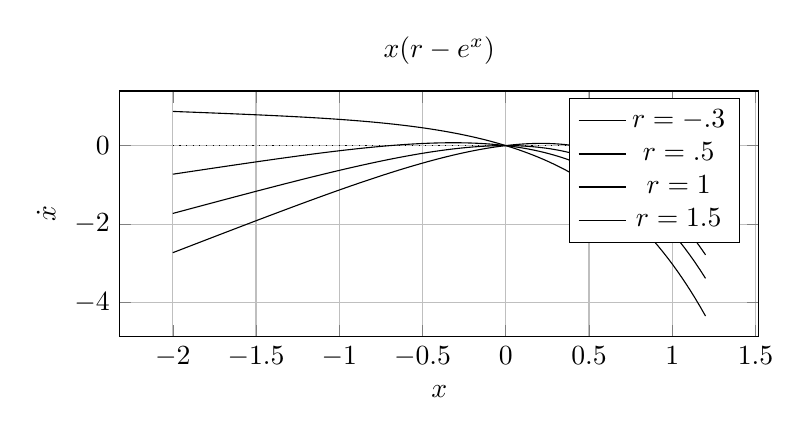
\begin{tikzpicture}
\begin{axis}[width=.8\textwidth,height=4.7cm,xlabel={$x$},ylabel={$\dot x$},title={$x(r-e^x)$},domain=-2:1.2,samples=100,grid=major,legend pos=north east]
\foreach \rr in {-.3,.5,1,1.5}{\addplot[no marks]{x*(\rr-exp(x))};\addlegendentryexpanded{$r=\rr$}}
\addplot[thin,dotted]coordinates{(-2,0)(1.2,0)};
\end{axis}
\end{tikzpicture}

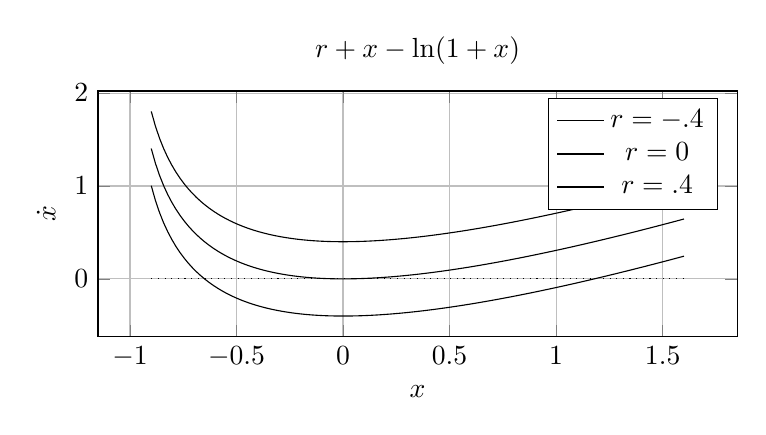
\begin{tikzpicture}
\begin{axis}[width=.8\textwidth,height=4.7cm,xlabel={$x$},ylabel={$\dot x$},title={$r+x-\ln(1+x)$},domain=-.9:1.6,samples=130,grid=major,legend pos=north east]
\foreach \rr in {-.4,0,.4}{\addplot[no marks]{\rr+x-ln(1+x)};\addlegendentryexpanded{$r=\rr$}}
\addplot[thin,dotted]coordinates{(-.9,0)(1.6,0)};
\end{axis}
\end{tikzpicture}

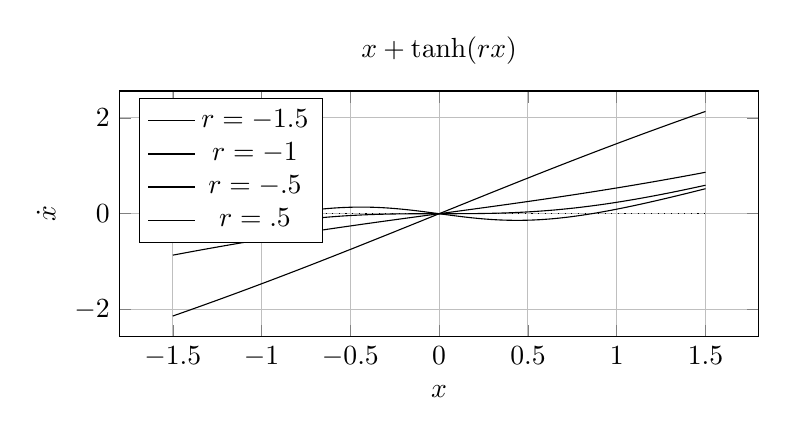
\begin{tikzpicture}
\begin{axis}[width=.8\textwidth,height=4.7cm,xlabel={$x$},ylabel={$\dot x$},title={$x+\tanh(rx)$},domain=-1.5:1.5,samples=120,grid=major,legend pos=north west]
\foreach \rr in {-1.5,-1,-.5,.5}{\addplot[no marks]{x+(exp(2*\rr*x)-1)/(exp(2*\rr*x)+1)};\addlegendentryexpanded{$r=\rr$}}
\addplot[thin,dotted]coordinates{(-1.5,0)(1.5,0)};
\end{axis}
\end{tikzpicture}
\end{center}
三幅是原函数本身的$\dot x$曲线, 与前面的局部分岔示意分开. 曲线在横轴上方表示向右运动, 下方表示向左; 交点是固定点.

